\chapter{Figures, Tables, and more}

In this chapter, figures, tables, and listings as available in this template are being introduced.\cite{NS2Manual}


\section{Figures}\label{sec:figures}

Figures should be frequently used throughout your thesis report, as they are a powerful instrument. Not only that one picture every two to three pages lightens up the work, a picture can even say more than a thousand words. However, note that a lonely figure is truly worthless. Make sure that you reference your figures in the text and that you explain them appropriately.

In the following, a set of useful commands for including figures into your work is introduced. Note that figures will be automatically placed by \LaTeX. You can rearrange figures be simply changing their position in the source code; however, you should not mess around with the figure placement options.


\subsection{Default yet Fancy Figures}\label{sub:simpleFigures}

Figures may require different display properties, so that a variety of different display styles are available. The main type of figures are illustrations. For these, the \cmd{\textbackslash{}fig} command is available. It has three parameters, which are the path to the picture, the caption, and the label. Labels of figures should have the prefix \cmd{fig:}. An example is shown in Figure~\ref{fig:simpleFigure}. The figure must be transparent, as it will be placed within a gray frame with a tiny border.

\fig{images/app_setup}{Figure with gray background box and border spacing. In this example, you also see what happens in case of a long caption.}{fig:simpleFigure}

In general, figures are displayed with a small inner spacing to the surrounding frame. As this may not be desired in some cases, there exists a version without additional spacing, \cmd{\textbackslash{}fignospacing}.


\subsection{The Frameless Variant}\label{sub:framelessFigures}

If you want to display photographs or illustrations, the surrounding frame and the gray background may be disturbing. Here, the command \cmd{\textbackslash{}fignoframe} jumps in and helps you out. The parameters are the same as described in Sect.~\ref{sub:simpleFigures}. See Fig.~\ref{fig:fignoframe} for a sample display.

\fignoframe{images/harvester}{Figure without surrounding frame and without gray background}{fig:fignoframe}


\subsection{Subfigures}\label{sub:subfigures}

When you start writing your evaluation and intend to display plots, having one plot per figure box is not a very handsome solution. Usually, you want to display multiple plots per figure box. This can be easily achieved using subfigures. In order to employ the neat and fancy boxing around your figures, use the \cmd{\textbackslash{}subfigbox}. As its first parameter, it takes a series of subfigures---using the \cmd{\textbackslash{}subfigure} command. Multiple rows are created using the \cmd{\textbackslash\!\textbackslash{}} command, automatic horizontal alignment is achieved via a \cmd{\textbackslash{}hfill} between adjacent figures in the same row. A possible layout is shown in Fig.~\ref{fig:trees}.

\subfigbox{
  \subfigure[complete]{\label{subfig:treeComplete}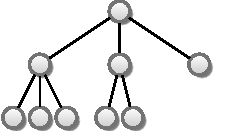
\includegraphics{images/tree_complete.pdf}}\hfill%
  \subfigure[min depth]{\label{subfig:treeMinDepth}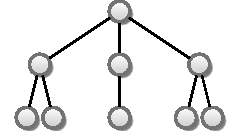
\includegraphics{images/tree_mindepth.pdf}}\hfill%
  \subfigure[full tree]{\label{subfig:treeFull}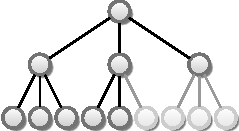
\includegraphics{images/tree_full.pdf}}%
}{Box with gray background intended to hold subfigures}{fig:trees}


%%
\section{Tables}\label{sec:tables}

Unfortunately, tables can be a pain in \LaTeX{} and have a clear tendency to look ugly. For this reason, we built the package \emph{tuhhtable}. A brief discussion of frequently used table pattern follow in dedicated subsections. 


\subsection{Simple Tables with Headings}\label{sub:simpleTables}

When creating tables, a couple of rules should be obeyed. Firstly, vertical lines are rarely helpful in tables. In contrast, they make a table harder to read in most cases, when people read from left to right. So try not to use them. To further support readability---while also hinting at eye candy---shaded rows are employed. To mark the end of a table and to separate the table body from the header, horizontal lines can be used. A recommended table layout is depicted in Table~\ref{tbl:simple}. Have a look at the source code of this document to understand how things work.\cite{MAC_Survey}

\begin{tuhhtable}
  \begin{tabular}[tp]{L{.3\textwidth}C{.3\textwidth}R{.3\textwidth}}
    \THc{1}{c}{Head 1} & \THc{1}{c}{Head 2} & \THc{1}{c}{Head 3} \\
    \THsub{1}{c}{sub 1} & \THsub{1}{c}{sub 2} & \THsub{1}{c}{sub 3} \\
    \abovebodyrule
    l1     & c1     & r1     \\\TRc
    l2     & c2     & r2     \\
    l3     & c3     & r3     \\\TRc
    \belowbodyrule
  \end{tabular}
  \caption{A simple table with a heading}
  \label{tbl:simple}
\end{tuhhtable}


\subsection{Special Table Elements}\label{sub:specialTableElements}

In case your are carrying out comparisons of, lets say, different algorithms, you might want to judge the quality of certain properties by symbols, such as '+', '-', or the like. Unfortunately, these symbols are not very fancy, so that we have defined a set of more eye-catchings ones. They are displayed in Table~\ref{tbl:elements}. Again, have a look at the source code of this document to understand how they can be used.

\begin{tuhhtable}
  \footnotesize\centering
  \begin{tabular}[tp]{L{.22\textwidth}C{.22\textwidth}C{.22\textwidth}C{.22\textwidth}}
    \THempty & \THc{1}{c}{Product 1} & \THc{1}{c}{Product 2} & \THc{1}{c}{Product 3} \\
    \abovebodyrule
    \TRh{1}{l}{has feature}  & \tblYes    & \tblYes  & \tblNo    \\\TRc
    \TRhc{1}{l}{usability}   & \tblGood   & \tblBest & \tblBad   \\
    \TRh{1}{l}{price}        & \tblNA     & \tblFair & \tblWorst \\\TRc
    \belowbodyrule
  \end{tabular}
  \caption{Special symbols for use in tables}
  \label{tbl:elements}
\end{tuhhtable}



\subsection{Advanced Tables}\label{sub:advancedTables}

Sometimes, a simple table layout as presented in the previous section is not sufficient. An example is shown in Table~\ref{tbl:advanced}. Hence, additional commands are available. 

% DECISION GUIDANCE TABLE
\begin{sidewaystable}
  \footnotesize\centering
  \begin{tabular}[htp]{lC{3.2cm}C{3.2cm}C{3.2cm}C{3.3cm}C{3.2cm}}
  \THempty    & \THc{1}{c}{Type I}   &
                 \THc{1}{c}{Type II}  &
                  \THc{1}{c}{Type III} &
                   \THc{1}{c}{Type IV}  &
                    \THc{1}{c}{Type V}  \\
%
  \TRx{6}{l}{Network Size}\\
  \abovebodyrule
  Small       & \tblWorst    & \tblGood     & \tblBest     & \tblBest     & \tblBad      \\\TRc
  Medium      & \tblFair     & \tblFair     & \tblGood     & \tblFair     & \tblFair     \\
  Large       & \tblBad      & \tblWorst    & \tblWorst    & \tblWorst    & \tblBest     \\
  \belowbodyrule
%
  \TRx{6}{l}{Density}\\
  \abovebodyrule
  Low         & \tblWorst    & \tblFair     & \tblBad      & \tblWorst    & \tblBad      \\\TRc
  Medium      & \tblFair     & \tblFair     & \tblFair     & \tblFair     & \tblGood     \\
  High        & \tblWorst    & \tblFair     & \tblGood     & \tblFair     & \tblGood     \\
  \belowbodyrule
%
  \TRx{6}{l}{Initial Fill Level}\\
  \abovebodyrule
  Low         & \tblFair     & \tblGood     & \tblBest     & \tblBest     & \tblGood     \\\TRc
  High        & \tblBad      & \tblBad      & \tblWorst    & \tblWorst    & \tblBest     \\
  \belowbodyrule
%
  \TRx{6}{l}{Variation of Initial Fill Levels}\\
  \abovebodyrule
  Low         & \tblBest     & \tblGood     & \tblBad      & \tblGood     & \tblBest     \\\TRc
  High        & \tblBest     & \tblBad      & \tblWorst    & \tblGood     & \tblBest     \\
  \belowbodyrule
%
  \TRx{6}{l}{Collisions and Packet Loss}\\
  \abovebodyrule
  Collisions / Yield &
    \tblYes / \tblWorst &
    \tblNo  / \tblBest &
    \tblNo  / \tblBest &
    \tblNo  / \tblBest &
    \tblYes / \tblFair     \\\TRc
  Packet Loss & \tblGood     & \tblFair     & \tblWorst    & \tblWorst    & \tblGood     \\
  \belowbodyrule
  \end{tabular}
  \caption{Characteristics of the TDMA schedules: Decision Guidance \cite{Renner:2008:Diploma}}
  \label{tbl:advanced}
\end{sidewaystable}



\section{Enumerations \& Co.}\label{sec:enumerations}

Feel free to use enumerations, itemizations, and the like to suit your needs. We have adjusted the itemization to match our slides class plus our color scheme. We thus discourage you from changing items or colors.



\section{Listings}\label{sec:listings}

For placing and typesetting listings, we encourage the use of the \emph{listings} package available for \LaTeX. Please have a look into the corresponding package manual. The facilitate the usage of this package, we have already set it up to follow the same look as the rest of our visual stuff. This includes the gray background, the frame, and appropriate colors. The package is automatically loaded by the template class and defines \emph{C++} as the default programming language---you are completely free to adjust the language, of course. A sample listing is displayed in Lst.~\ref{lst:sampleListing}. Note that all listings should have labels with the prefix \cmd{lst:} and should be referenced in the text. Besides complete listings, we have defined the command \cmd{\textbackslash{}cmd}, which display its first parameter text in monospace font.

\begin{lstlisting}[label=lst:sampleListing,caption={A simple C++ program for reading in positions}]
#include <iostream>                                                                       
#include <vector>                                                                         
#include <inttypes.h>                                                                     

using namespace std;

/* 2-D positions */
typedef struct pos_s {
        int16_t  x, y;
} pos_t;

int main(void)
{
        uint16_t       numData;
        vector<pos_t>  v;
        pos_t          tmp;

        /* read numData 2-D points */
        cin >> numData;
        for (unsigned i = 0; i < numData; i++) {
                cin >> tmp.x >> tmp.y;
                v.push_back(tmp);
        }
        cout << "read " << numData << " points" << endl;

        /* process data */
        process(v);

        return 0;
}
\end{lstlisting}
